\documentclass[a4paper,10pt]{article}

\usepackage[english]{babel}
\usepackage[utf8]{inputenc}

\usepackage{amsmath,amssymb}
\usepackage{color,graphicx}
\usepackage{cprotect}

\usepackage{listings}

\title{RE atlas manual}
\author{Anders A. Søndergaard}

\def\changemargin#1#2{\list{}{\rightmargin#2\leftmargin#1}\item[]}
     \let\endchangemargin=\endlist 

\begin{document}

\maketitle

\tableofcontents

\section{Brief introduction to the REatlas and some terminology}

The REatlas is a computer program designed to convert
weather data into production profiles for wind and photovoltaics (solar) power
technologies. It has a server part and a client part. The server part
runs on a big computer, located at Aarhus University, and does the actual computation, while the client
part can be run on any personal computer.

The REatlas server is what is known as a \emph{Remote Procedure Call} (RPC)
server, i.e. it is a server that allows you to execute function calls
on it, as if they were executed on the client computer.

The REatlas client is simply a library for setting up and handling
the connection and underlying protocol for the RPC server.

\subsection{Cutouts}

The weather data is global and consists of large arrays of meterological
parameters from the CFSR\cite{cfsr}, such as wind speed and sun light intensity.
Each entry, or \emph{grid cell} in such an array is identified by the latitude and longitude of its center, and it represents a
geographical localtion somewhere in the world.

Because of the size of the data set, you
typically will not want to work with all of it at the same time,
since it will take several days to convert it all to production timeseries.

Therefore, you cut out some part of the world that you are interested in.
This could for example be Europe, USA, China or Denmark.
The smaller the area, the faster the conversion.

A \emph{cutout} is such a selection of an area of interest. 
Cutouts can either be box shaped (with sides of constant latitude/longitude) or a collection of individual grid cells.

\subsection{Aggregation and capacity layouts}

The main purpose of the atlas is to generate time series
for regions of interest, e.g. countries or continents.

When all the grid cells in a cutout are converted,
a new grid (i.e. array) of production values are created
with the same dimensions as the raw data arrays.

To get a time series (under the \emph{copper plate assumption})
of the region of interest, a \emph{capacity layout} is needed.
This is simply an array with the same shape as the
cutout, where each grid cell is assigned a \emph{weight}.
This weight could e.g. be the installed capacity in MW or the number
of turbines/solar panels per cell.

An \emph{aggregation} is the process of multiplying all grid cells
with the corresponding weight in a capacity layout and summing up
the resulting values.

If the capacity layout e.g. contains 1's everywhere in the region,
and 0's eleswhere, a time series for the region will be obtained
with capacity uniformly distributed across it.

\section{Installing the client}

The client can be downloaded from github.com/AUESG.
It requires Python and Numpy to run, and optionally scipy (for Matlab support)
and pyshp (for GIS support). Python can be downloaded from python.org,
and Numpy can be downloaded from numpy.org.

To use the REatlas, you must have an account on the server.

To connect to the server, you must be on the Aarhus University
internal network. If you're running the client from outside
the intranet, you have 3 options:

\begin{itemize}
     \item Tunnel through pepsi (you need an account on pepsi for this):

          \verb+ssh -L 65535:pepsimax.imf.au.dk:65535 pepsi.imf.au.dk+
     \item Tunnel through NFIT's LogInFArm (you need an NFIT account for this):

          \verb+ssh -L 65535:pepsimax.imf.au.dk:65535 lifa.phys.au.dk+
     \item Use the AU VPN solution (you need an AU VPN account for this).

\end{itemize}
Note that if you use the ssh options to tunnel through AU firewalls,
you should connect the REatlas client to "localhost" instead of using
the server name.


\section{Client commands}

The client consists of a client library, and a collection of command line
utilities based on the library. These command line utilities can be
used without any programming effort.


%\begin{lstlisting}
%print("Hello, world!");
%\end{lslisting}

\subsection{Available commands}

\subsubsection{cmd\_list\_cutouts.py} Get a list of existing cutouts.
\ \\ \ \\ \cprotect\framebox{\begin{minipage}{\textwidth}
Example: \verb+python cmd_list_cutouts.py servername+
\end{minipage}}
\subsubsection{cmd\_get\_cutout\_metadata.py} Download metadata for a REatlas cutout in either .npz, .csv, .mat or .shp format. npz is a numpy (Python) format, .csv is a comma separated text file, .mat is for Matlab files, and .shp is the Esri shape file format, used by e.g. QGis or ArcMap.
\ \\ \ \\ \cprotect\framebox{\begin{minipage}{\textwidth}
Example: Download all metadata for the Denmark cutout under auesg to a csv file.
 \begin{verbatim}
python cmd_get_cutout_metadata.py servername Denmark \
/path/to/data/Denmark.csv --cutoutuser auesg
\end{verbatim}
\end{minipage}}
\subsubsection{cmd\_convert\_and\_aggregate\_wind.py} Script for starting a wind conversion on a cutout. Requires a capacity layout in either .npy, .csv, .mat or .shp format.
\ \\ \ \\ \cprotect\framebox{\begin{minipage}{\textwidth}
Example: Convert wind for Denmark with a Vestas 90 3 MW turbine offshore
and a Siemens SWT 2.3 MW turbine onshore, and aggregate with two layouts (in different formats):
\begin{verbatim}
python cmd_convert_and_aggregate_wind.py servername Denmark \ 
--cutoutuser auesg --name Windconversion1
TurbineConfig/Siemens_SWT_2300kW.cfg \
TurbineConfig/Vestas_V90_3MW.cfg \ 
layout1.shp layout2.csv
\end{verbatim}
\end{minipage}}
\subsubsection{cmd\_convert\_and\_aggregate\_PV.py} Script for starting a PV conversion on a cutout. Requires a capacity layout in either .npy, .csv, .mat or .shp format.
\ \\ \ \\ \cprotect\framebox{\begin{minipage}{\textwidth}
Example: Convert PV for Denmark with a Scheuten 215IG solar panel,
with a fixed orientation:
\begin{verbatim}
python cmd_convert_and_aggregate_PV.py servername Denmark \ 
--cutoutuser auesg --name PVconv1 \
SolarPanelData/Scheuten215IG.cfg \
orientation_examples/constant.cfg \
layout.npy
\end{verbatim}
\end{minipage}}
\subsubsection{cmd\_get\_result.py} Waits for and downloads the result of a conversion and aggregation.
\ \\ \ \\ \cprotect\framebox{\begin{minipage}{\textwidth}
Example: Download the result from the above PV conversion to a matlab file.
\begin{verbatim}
python cmd_get_result.py servername job_id PVconv1 PVresult.mat
\end{verbatim}
\end{minipage}}
\subsubsection{cmd\_create\_CFSR\_rectangular\_cutout.py} Script for cutting out a rectangular region. Takes southwesternmost and northeasternmost point in the rectangle as arguments. Note: This takes very long time, and you may not be allowed to execute this function.
\ \\ \ \\ \cprotect\framebox{\begin{minipage}{\textwidth}
Example: Create a cutout that contains Germany:
\begin{verbatim}
python cmd_create_CFSR_rectangular_cutout.py servername \ 
Germany 46.6 3.5 55.5 16.6
\end{verbatim}
\end{minipage}}
\subsubsection{cmd\_create\_CFSR\_pointwise\_cutout.py} Script for cutting out a pointwise region. Takes a list of GPS coordinates of points to cut out. Note: Making a new cutout takes about 24 hours, where the server cannot be used for anything else. Regardless of cutout size.
\ \\ \ \\ \cprotect\framebox{\begin{minipage}{\textwidth}
Example: Create a cutout that contains Aarhus, Copenhagen and Rome:
\begin{verbatim}
python cmd_create_CFSR_pointwise_cutout.py servername \ 
AarhusCopenhagenRome 56.2,10.2 55.7,12.5 42.0,12.5
\end{verbatim}
\end{minipage}}
\subsubsection{cmd\_job\_list.py} Get a list of your currently scheduled jobs.
\ \\ \ \\ \cprotect\framebox{\begin{minipage}{\textwidth}
Example: See your queued jobs and ETA's along with the total workload of the server:
\begin{verbatim}
python cmd_job_list.py servername
\end{verbatim}
\end{minipage}}
\subsubsection{cmd\_cancel\_jobs.py} Cancel jobs on the REatlas server. Note: Running jobs cannot be canceled.
\ \\ \ \\ \cprotect\framebox{\begin{minipage}{\textwidth}
Example: Cancel all your jobs:
\begin{verbatim}
python cmd_cancel_jobs.py servername
\end{verbatim}
\end{minipage}}
\subsubsection{cmd\_shutdown\_atlas.py} Command for shutting down the atlas. All pending jobs are executed before the atlas closes down. Only useful for maintenance tasks. Can only be run by privileged users.
\ \\ \ \\ \cprotect\framebox{\begin{minipage}{\textwidth}
Example:
\begin{verbatim}
python cmd_shutdown_atlas.py servername
\end{verbatim}
\end{minipage}}

\subsection{Note about working with capacity layouts and shapefiles}

A capacity layout is an array in the same shape as the layout for
which it is meant to be applied.

The command line utility \verb+cmd_get_cutout_metadata.py+ downloads
arrays in this shape, containing latitude, longitude, on/offshore and
depth/height data. You can repurpose these arrays for making
capacity layouts.

When you download the metadata as a shapefile, you can edit
this shapefile (e.g. with ArcGis or quantum gis, qgis).
The shapefile contains points representing the center of each grid cell.
The attribute table contains the field ``CAPACITY''.
By changing this field, you can assign a capacity to each grid cell
and use the shapefile as input capacity layout. See figure \ref{fig:qgis}.

\begin{figure}[h]
\begin{center}
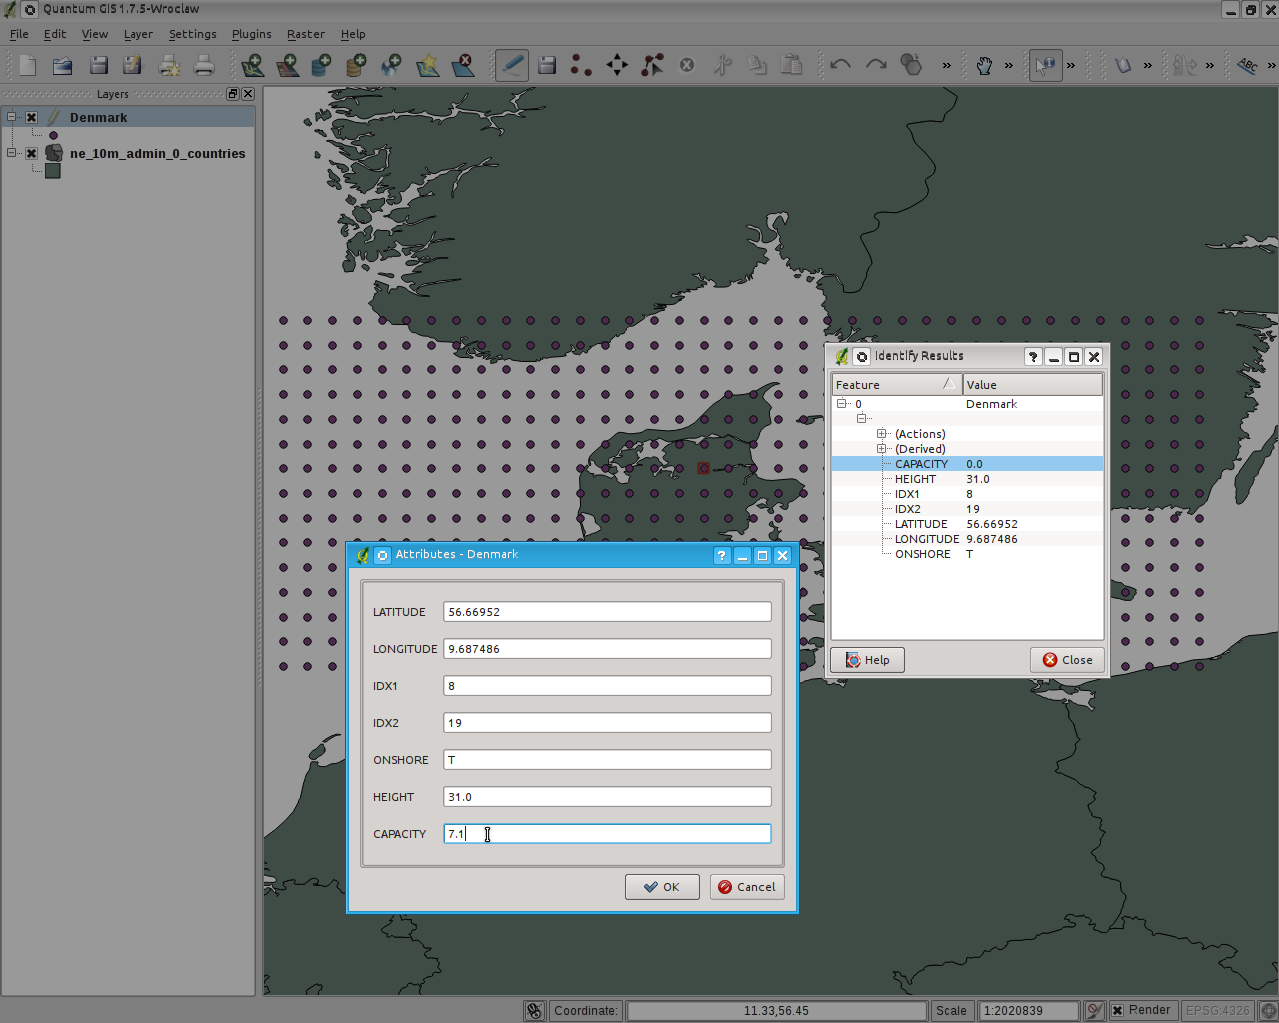
\includegraphics[width=\textwidth]{qgis.png}
\end{center}
\caption{Using qgis to set the capacity of a grid cell to 7.1.}
\label{fig:qgis}
\end{figure}


\section{Usage examples and exercises (client library)}

In this section, a few excercises in using the REatlas client library are given.
A script that solves the problems can be found in the exercises.py file.

Before trying the exercises, you should have some sort of network connection
to the REatlas, along with an account.

Using interactive python (IPython) is recommended, or alternatively
writing a Python script.

Note that the RPC functions require their full keyword arguments
specified. I.e. positional arguments does not work.
The reason for this has something to do with the underlying RPC protocol 
for sending function arguments.


\subsection{Exercise 1: Familiarize youself with the atlas}

In this exercise, you will connect to the REatlas and take a look around.

\begin{enumerate}
     \item Download the REatlas client software from github.com/AUESG.
     \item Login to the REatlas (use the connect\_and\_login function).
     \item Succesfully call the echo() and generate\_error() functions.
           generate\_error() will give you an example error message.
     \item Get a list of all the cutouts that are available on the server.
           How much space does Europe and Denmark take up?
           (answer: 133 GB and 3 GB, respectively)
     \item Download all the metadata for Europe and/or Denmark.
           (Hint: use the prepare\_cutout\_metadata() and download\_file() functions).
           How many points are there in the Europe/Denmark cutout?
           (Hint: derive this from the shape of the latitude/longitude array.
           Answer: 21279 and 600, respectively)
      \item Start a dummy job (a job that does nothing for 15 seconds) on
           the server, and read the email you get when it finishes.
           Start another dummy job without receiving an email when it finishes.
           (hint: use the notify\_by\_mail() function).

      \item Use the wait\_for\_job() function to wait for a dummy job to finish.
           How could the wait\_for\_job() function be useful (in a script)?

\end{enumerate}

\subsection{Exercise 2: Wind conversion}

In this exercise, you will perform a wind conversion on the REatlas server,
and you will create example capacity layouts.
     
\begin{enumerate}
     \item Find out how much power a Vestas V90 3MW turbine would have produced
           on January 13, 1992 at 05.00 UTC if it were placed
           on 56.9 degrees latitude, 7.5 degrees longitude.
           (answer: 2.9 MW). According to the REatlas (and to Google maps),
           is this point onshore or offshore?
           According to the REatlas, how deep is the water in this grid cell?
           (answer: 29 meters)

           Hints:
           \begin{enumerate}
               \item Load the Vestas V90 3MW config file with the
                    REatlas client provided turbineconf\_to\_powercurve\_object() function.
               \item Make a capacity layout for Denmark/Europe
                     consisting of only 0's except for the grid cell
                     containing 56.9 degrees latitude, 7.5 degrees longitude.
                     This grid cell should contain a 1.
                     Applying this capacity layout effectively gives
                     the timeseries for that single grid cell.

                \item You can find the index of that grid cell by using the
                     translate\_GPS\_coordinates\_to\_array\_indices() function
                     provided by the REatlas client on the metadata for the cutout.
                     For Denmark, 56.9,7.5 degrees has the index (9,12).
                \item Upload the capacity layout with upload\_file()
                \item Select the cutout you want to work with with the 
                     select\_cutout() function.
                \item Start a wind conversion with convert\_and\_aggregate\_wind().
                \item Download the resulting file, and use the ``dates'' metadata file to find the timeseries index for 1992 at 05:00 utc.
                     numpy.where and datetime.datetime will be useful for this purpose.
           \end{enumerate}
      \item Get a normalized time series of wind production for Denmark in the 
           period 1979-2010 for a Vestas V90 3 MW turbine if it were
           distributed uniformly in all onshore grid cells.
      \item Get two normalized timeseries using only one call to the
           convert\_and\_aggregate\_wind() function. Use the capacity layouts
           from the previous two exercises.

\end{enumerate}

\subsection{Exercise 3: PV conversion}

In this exercise, you will perform a PV conversion on the REatlas server,
and you will create example capacity layouts.
You will compare a solar cell mounted in a fixed position to 
a distribution of orientations, and to a solar panel that tracks the sun.


\begin{enumerate}
     \item As an approximation, assume that a side of a house can either face
          east, west or south (and that nobody installs solar panels on a north facing side), and that all roofs have a slope of 45 degrees.
          Perform a PV conversion with the Scheuten 215IG roof-mounted panel
          distributed equally in all Danish onshore grid cells
          with a distribution of 33 \% of panels facing west, 33\% facing east
          and 34\% facing south (azimuth: 90, -90 and 0 degrees, respectively).
          
          Hint: This follows the same procedure as for wind conversion,
          except panel config files are loaded with the
          solarpanelconf\_to\_solar\_panel\_config\_object() function,
          and that solar panel orientations must also be specified before
          calling convert\_and\_aggregate\_pv().

          You can add orientations to PV conversion with the add\_*\_orientation\_function() functions.
          Each call to convert\_and\_aggregate\_pv resets the choice of orientations. This is also true for reset\_orientations().
          You can use the latter for undoing mistakes.

     \item Perform another PV conversion and aggregation for onshore Denmark
           where all panels point straight south and have a slope of 32 degrees.
           Perform another PV conversion and aggregation for onshore Denmark
           where each panel tracks the sun.
      \item Plot (with e.g. matplotlib.pyplot) sample days for the three
           different conversions and compare them.
\end{enumerate}


\section{Available functions}

\subsection{Overview of client built-in helper functions}

Apart from providing the \verb+REatlas+ object, the REatlas client
also provides these functions:

\subsubsection{turbineconf\_to\_powercurve\_object()}

Used for loading turbine configuration files in as objects. These objects
can be used as arguments in wind conversion calls.

\subsubsection{solarpanelconf\_to\_solar\_panel\_config\_object()}

Used for loading solar panel configuration files in as objects.
These objects can be used as arguments in PV conversion calls.

\subsubsection{translate\_GPS\_coordinates\_to\_array\_indices()}

Can be used to find the grid cell nearest some point given by GPS coordinates.

\subsubsection{Misc.}

Apart from this, the client also provides a few helper functions in the
REatlas object itself. These are:

\begin{itemize}
     \item \textbf{download\_file()} Used to download files from the server.
     \item \textbf{upload\_file()} Used to upload files to the server.
     \item \textbf{connect\_and\_login()} Used in interactive mode to connect and login in one go. If you just \verb+connect()+, the connection times out faster than you can type in your login details. This also calls \verb+build_functions()+.
     \item \textbf{build\_functions()} Initially, the client does now know about the RPC functions available. This method queries the server for available RPC functions and adds them as local class methods.
     \item \textbf{add\_pv\_orientations\_by\_config\_file()} Parses a configuration file of orientations and adds them via the add\_*\_orientation\_function() RPC functions. 
\end{itemize}


\subsection{Overview of RPC methods}

The following functions are defined on the REatlas server,
and can be called as is they were on the client computer.

To call them, you must first call the \verb+REatlas.build_functions()+ or
\verb+REatlas.connect_and_login()+ methods. 

\begin{changemargin}{-1.5cm}{1.5cm}
\subsubsection{\_select\_current\_file()}


\begin{verbatim}
 _select_current_file(filename,username="",intent="")

               filename: Filename to select.
               username: If given, select a file in that users directory
                         instead of your own.
               intent: If given and equal to "download",
                       return an error if the file does not exist.

          Selects which binary file to send to or receive from the server.
          These are send as raw binary instead of through JSON-RPC.

          
\end{verbatim}
\subsubsection{delete\_file()}


\begin{verbatim}
 delete_file(filename,username="")

               filename: Name of file to delete.
               username: If given, delete the file in this users directory instead of your own.
          
          Example:
               delete_file(filename="foo.npy",username="someguy")

          Delete foo.npy under someguys folder.

          Returns True on success.
          
\end{verbatim}
\subsubsection{list\_files()}


\begin{verbatim}
 list_files(username=""):

          Return a list of your files and their sizes in bytes.

          Arguments:
               username: If given, list this users files instead of your own.

          Example:
               list_files()
          returns a list of all your files on the server.

          
\end{verbatim}
\subsubsection{login()}


\begin{verbatim}
 Log in to the server with supplied credentials. Returns True
          on success, and False on invalid credentials.
          
          Keyword arguments:
               username
               password
          
          It is a good idea to login immediately after a connection is made,
          as the server times out very quickly if no user is logged in.
\end{verbatim}
\subsubsection{job\_priority()}


\begin{verbatim}
 Set or get current priority level.
          
          job_priority(priority=None) -> int

          Sets priority level of current session to priority.
          Any jobs submitted afterwards will have this priority.
          Priority must be 0, 1 or 2. The higher the number, the higher the priority.
          If not specified, only return current priority level.

          Note: If priority exceeds the users max_priority setting,
          this call sets the priority level to max_priority.
          
          
          Examples:
               job_priority()
               1

          Your jobs will be submitted with job priority 1.

               job_priority(priority=2)
               1
          You tried to set a priority level of 2, but your maximum allowed
          priority is 1. 
          
          
\end{verbatim}
\subsubsection{notify\_by\_mail()}


\begin{verbatim}
 Gets/sets notify option of current session
         
          notify_by_mail(s,notify=None) -> Bool

          Notify must be None, False or True. If None,
          only return current notification setting.
          If True or False, set current notification setting
          to True or False, respectively.

          If the notification setting is True, jobs you create will send
          you a notification email when done. 
          
          Example:
               notify_by_mail(notify=False)
               False
          Jobs you submit during this session will no longer send an
          email to you when done.
          
          
\end{verbatim}
\subsubsection{\_get\_available\_methods()}


\begin{verbatim}
 Return a list of JSON-RPC methods (functions) that
          the server accepts. 
\end{verbatim}
\subsubsection{\_get\_method\_docstrings()}


\begin{verbatim}
 Returns a dictionary of Python docstrings for the
          methods provided by the server. 
\end{verbatim}
\subsubsection{\_get\_server\_endianness()}


\begin{verbatim}
 Gets the byte order used by the server CPU 
          
          _get_server_endianness() -> str

          Returns:
               'little' if the server is a little endian machine or
               'big' if the server is a big endian machine.
\end{verbatim}
\subsubsection{echo()}


\begin{verbatim}
 echo(message=""):
               returns message. 
\end{verbatim}
\subsubsection{generate\_error()}


\begin{verbatim}
 Generates an example error. 
\end{verbatim}
\subsubsection{list\_cutouts()}


\begin{verbatim}
 Returns a list of tuples with cutouts and used space.
          
               list_cutouts(all_users=False,loaded=False)

          If all_users is True, then list cutouts of all users
          instead of only the current user.

          If loaded is True, then list the cutouts loaded in the ramdisk
          instead of those on the hard disk.
          This requires super user privileges.

          Each cutout is given as user/cutout_name. Entries containing
          just user without /cutout_name gives the total space used by that users cutouts. 
\end{verbatim}

\subsubsection{submit\_dummy\_job()}


\begin{verbatim}
 
          Queue a job on the server that does nothing for 15 seconds.
          No arguments.
          
\end{verbatim}
\subsubsection{get\_queued\_job\_time()}


\begin{verbatim}

          Returns the estimated time (in seconds) of work currently
          in the queue by user name as a dictionary. 

          If you're not privileged, it only returns the estimated time
          your jobs account for and the total time. 
          
          Example:
               get_queued_job_time()
               {u'TOTAL': 3600,
                u'jens': 180}
          If your username is jens, you have jobs worth of 180 seconds in the queue.
          There is a total of 3600 seconds of jobs currently waiting.
          
          
\end{verbatim}
\subsubsection{get\_estimated\_time\_before\_completion\_of\_jobs()}


\begin{verbatim}
 Get estimated time for a specific job to be done.
          
          Considering all queued jobs, return the estimated
          time (in seconds) before a specific job completes.

          Arguments (optional):
               job_id: ID of the job to get an estimate for.
                       If not given, return a list of time left for all jobs.

          If job_id is specified and no job has that job id
          (e.g. if it is finished), then this returns None.

          Note: time estimates are rather rough.

          Example:
               timings = get_estimated_time_before_completion_of_jobs()
               timings[33]
               500

          Here you see that job 33 is estimated to be done in 500 seconds.
          If this is larger than the time estimate for job 33, this means
          that the job is waiting for other jobs to finish.
          
\end{verbatim}
\subsubsection{list\_queued\_jobs()}


\begin{verbatim}
 Get a list of jobs in queue and some info.

          No arguments.

          Returns a list of jobs.
          If you are not privileged, you will only see your own jobs.
          Each entry is a dictionary with the keys:
               user: Username of the job owner.
               name: Name of the job.
               job_id: ID of the job.
               time_estimate: Estimated job running time (in seconds).
               ETA: Estimated time left before job completion (in seconds).

          Note: time estimates are rather rough.
          
\end{verbatim}
\subsubsection{wait\_for\_job()}


\begin{verbatim}
 Waits (i.e. doesn't return before) job completes.
     
          Arguments:
               job_id: Id of the job to wait for.
               timeout: Wait for at most this many seconds.
                    Defaults to 3600 (1 hour).
          
          When the waiting is over, 
          the return value is True if the job is done, False otherwise. 
          
          Example:
               wait_for_job(job_id=33)
               [... nothing happens until job 33 is done,
                    or an hour has passed ...]
               False

          Indicates that the job is not done yet, and you should call
          wait_for_job again if you want to wait for it.
          
\end{verbatim}
\subsubsection{cancel\_jobs\_of\_user()}


\begin{verbatim}
 Cancel all jobs of a user.
          
          Without any arguments, this function cancels all your jobs
          that are waiting in the queue.

          Arguments:
               username: If given, cancel the specified users jobs instead. 
\end{verbatim}
\subsubsection{translate\_GPS\_coordinates\_to\_CFSR\_index()}


\begin{verbatim}
 Find the CFSR indices of given GPS coordinates.
          
          translate_GPS_coordinates_to_CFSR_index(latitudes,longitudes)
               -> [CFSRindex_0, CFSRindex_1]

          Arguments:
               latitudes and longitudes are lists of numbers corresponding
               to the requested GPS coordinates.
               latitudes[i] and longitudes[i] should be the GPS latitude
               and longitude of point i.

          Returns: A 2-element list of lists of first and second CFSR indices.
          I.e. [[latitude0,latitude1,...], [longitude0,longitude1,...]]. 
          
          Example:
               translate_GPS_coordinates_to_CFSR_index(latitudes =[55,56],
                                                       longitudes=[7 , 6])
          [[464, 467], [22, 19]]

          This shows that 55 degrees north, 7 degrees east has the CFSR
          index 464,22 and the point 56,6 has index 467,19
          
\end{verbatim}
\subsubsection{cutout\_CFSR\_rectangular\_by\_GPS\_coordinates()}


\begin{verbatim}
 Cut out a rectangle of the CFSR data based on GPS coordinates.
          
          Functionally identical to CFSR_rectangular_cutout_by_CFSR_indices,
          but southwest and northeast should be GPS coordinates instead of 
          CFSR indices. The first entry in southwest/northeast is the latitude
          and the second is the longitude.
         
          This method simply translates the GPS coordinates to
          CFSR indices via the translate_GPS_coordinates_to_CFSR_index method
          before calling CFSR_rectangular_cutout_by_CFSR_indices.
          
\end{verbatim}
\subsubsection{cutout\_CFSR\_rectangular\_by\_CFSR\_indices()}


\begin{verbatim}
 Cut out a rectangle of the CFSR data based on CFSR indices.

               CFSR_rectangular_cutout_by_CFSR_indices(name,southwest,northeast,
                    firstyear=None,lastyear=None,firstmonth=None,lastmonth=None,
                    double=False,nowind=False,nopv=False) -> int or None

               name: Name of the cutout
               southwest, northeast: lists of CFSR indices of the southwesternmost
                    and northeasternmost points in the rectangle.
                    These should be 2-element lists of integers.
               firstyear,firstmonth,lastyear,lastmonth: If specified,
                         these set the temporal range of the cutout.
                         E.g. if firstyear=2000, only use from 2000 and onwards.
                         If lastyear=2004, only use data before 2004.
               double: If True, dump the cutout in double precision. This requires
                       super user privileges.
               nowind: If True, don't cut out data needed for wind conversion
               nopv: If True, don't cut out data needed for photovoltaics conversion

              Returns the job id of the cutout job submitted to the queue,
              or None if the queue is closed or full.
                       
\end{verbatim}
\subsubsection{cutout\_CFSR\_individual\_points\_by\_GPS\_coordinates()}


\begin{verbatim}
 Cut out individual CFSR grid cells based on GPS coordinates.
          
          CFSR_individual_cutout_by_GPS_coordinates(name,latitudes,longitudes,
               firstyear=None,lastyear=None,firstmonth=None,lastmonth=None,
               double=False,nowind=False,nopv=False)
     
          Translate latitudes and longitudes to CFSR indices with
          translate_GPS_coordinates_to_CFSR_index() and call
          CFSR_individual_cutout_by_CFSR_indices() with the given arguments
          and the translated indices.
          
          
          Example:
               cutout_CFSR_individual_points_by_GPS_coordinates(name="test",
                    latitudes=[55,56],longitudes=[7.5,9])

               cuts out two points 55,7.5 and 56,9 in GPS coordinates.
          
          
\end{verbatim}
\subsubsection{cutout\_CFSR\_individual\_points\_by\_CFSR\_indices()}


\begin{verbatim}
 Cut out individual CFSR grid cells based on CFSR indices.

          CFSR_individual_cutout_by_CFSR_indices(s,name,
               first_indices,second_indices,
               firstyear=None,lastyear=None,firstmonth=None,lastmonth=None,
               double=False,nowind=False,nopv=False) -> int or None

               name: Name of the cutout
               first_indices,second_indices: Arrays of CFSR first and second indices.
                    The i'th point should have index first_indices[i],second_indices[i].
               firstyear,firstmonth,lastyear,lastmonth: If specified,
                         these set the temporal range of the cutout.
                         E.g. if firstyear=2000, only use from 2000 and onwards.
                         If lastyear=2004, only use data before 2004.
               double: If True, dump the cutout in double precision. This requires
                       super user privileges.
               nowind: If True, don't cut out data needed for wind conversion
               nopv: If True, don't cut out data needed for photovoltaics conversion

              Returns the job id of the cutout job submitted to the queue,
              or None if the queue is closed or full.  
              
              Example:
               cutout_CFSR_individual_points_by_CFSR_indices(name="test",
                    first_indices=[464, 467], second_indices=[22, 19]);

                    cuts out the CFSR points 464,22 and 467,19 and give
                    it the name "test".
              
\end{verbatim}
\subsubsection{delete\_cutout()}


\begin{verbatim}
 Delete a cutout
          
          delete_cutout(cutoutname,username=None)

          Delete cutout called cutoutname. If username is not specified, a cutout
          under the current user is deleted.
          If username (a string) is specified, delete that users cutout
          with that name.

          Deleting other users cutouts require super user privileges.
          
          Example:
               delete_cutout(cutoutname="test")

               deletes your cutout named test.
          
          
\end{verbatim}
\subsubsection{prepare\_cutout\_metadata()}


\begin{verbatim}
 Makes available all meta data for a given cutout in your server directory.
          
          Arguments:
               cutoutname: Name of the cutout to get data from.
               username: If given, find the cutout under this users cutouts
                         instead of your own.
          
          On successful return, a file named meta_<cutoutname>.npz will
          be available for download in your folder.

          It is a zipped file with the following numpy arrays:

               latitudes,longitudes: Contains latitudes and longitudes (in degrees)
                                     of each point in the cutout.
                                     The i,j'th entry corresponds to the i,j'th
                                     point in the cutout.

               dates: Timestamps of each hour in the cutout.
                      The i'th entry here corresponds to the i'th hour in the cutout. 

               onshoremap: A map of onshore points.
                           Cell i,j contains 1 if the point is onshore, 0 otherwise.

               heights: The height in of the grid cell.
                        Negative numbers indicate below sea level.
                        These values are derived by interpolating the
                        GEBCO 30 arc minute grid at the center of each grid cell.

          The .npz file can be opened directly by numpy's load() function.
          
\end{verbatim}
\subsubsection{\_get\_unique\_npy\_file()}


\begin{verbatim}

          Generate a file with a unique name in your directory.
          The filename will end with ".npy".
          
          This function could be useful if you do a lot of
          conversion + aggregation jobs for automatic name generation.

          Returns the name of the file, including the .npy extension. 
\end{verbatim}
\subsubsection{select\_cutout()}


\begin{verbatim}
 Selects a cutout for doing conversions.

          Arguments:
               cutoutname: Name of the cutout to select.
               username: If given, select this users cutout.

          All conversions will be done on the selected cutout.
          
\end{verbatim}
\subsubsection{get\_selected\_cutout()}


\begin{verbatim}
 Returns a tuple (cutoutname, username) for the currently selected cutout. 
\end{verbatim}
\subsubsection{convert\_and\_aggregate\_wind()}


\begin{verbatim}
 Submit a wind conversion and aggregation to job queue.

          Returns the job number of the conversion in the job queue.

          Arguments:
               result_name: Name of file for storing the result.
               onshorepowercurve: A powercurve object for use onshore.
               offshorepowercurve: A powercurve object for use offshore.
               capacitylayouts: A list of file names in your folder containing
                                capacitylayouts to apply.
                                These should all be numpy (.npy) files.
               save_sum: If true, store the sum of production of all grid cells
                         in result_name + "_sum.npy" in your folder on the server.
                         If save_sum is true, the list of capacity layouts can
                         be empty, in which case only the sum is calculated.
               onshoremap: If given, use this named .npy file in your server folder
                           as an onshoremap instead of the default CFSR land sea mask.
               nthreads: If given, run the conversion and aggregation
                         with this many threads. Requires privileges to set.
               worksize: If given, each thread converts/aggregates this many
                         hours at a time. Requires privileges to set.

     
          The result is stored in your folder on the server with the name
          you gave as parameter result_name. It is a numpy array with a number
          of timeseries equal to the number of layouts you specified.
          To get e.g. hour 100 for layout number 2, use result_name[99][1]. 

          A powercurve object is a dictionary with three keys: HUB_HEIGHT, V and POW.
          The value for HUB_HEIGHT is the hub height in meters above ground.
          The values for V and POW are equal length lists of numbers.
          POW[i] is the power output for a wind speed V[i].
          The V's must be increasing for the linear interpolation routine to work,
          and be in units of meters per second.

          Note: To get production values between 0 and 1, send scaled down power curves!
          The timeseries are simply a weighted sum over production in the entire cutout,
          with the layout cells as weights. The unit of the sum is the unit of the layout
          times the unit on the second axis of the power curve.
          
\end{verbatim}
\subsubsection{reset\_orientations()}


\begin{verbatim}
 Reset the list of solar panel orientation functions. 
\end{verbatim}
\subsubsection{add\_constant\_orientation\_function()}


\begin{verbatim}
 Add a constant orientation to the list of PV panel orientations
          for PV conversions. 
          
          Arguments:
               slope: The slope, i.e. angle between panel and ground, in degrees.
               azimuth: The east-west angle of the panel, in degrees.
                        Westward direction is positive, eastward negative.
               weight: Factor to apply to the result of the conversion
                       with this orientation.
          
\end{verbatim}
\subsubsection{add\_horizontal\_axis\_tracking\_orientation\_function()}


\begin{verbatim}
 Add a horizontal axis tracking orientation to the list of
          PV panel orientations for PV conversions. 
          
          Arguments:
               slope: The constant slope, i.e. angle between panel and ground, in degrees.
               weight: Factor to apply to the result of the conversion
                       with this orientation.
          
\end{verbatim}
\subsubsection{add\_vertical\_axis\_tracking\_orientation\_function()}


\begin{verbatim}
 Add a vertical axis tracking orientation to the list of
          PV panel orientations for PV conversions. 
          
          Arguments:
               azimuth: The constant east-west angle of the panel, in degrees.
                        Westward direction is positive, eastward negative.
               weight: Factor to apply to the result of the conversion
                       with this orientation.
          
\end{verbatim}
\subsubsection{add\_full\_tracking\_orientation\_function()}


\begin{verbatim}
 Add a full axis tracking orientation to the list of
          PV panel orientations for PV conversions. 
          
          Arguments:
               weight: Factor to apply to the result of the conversion
                       with this orientation.
          
\end{verbatim}
\subsubsection{convert\_and\_aggregate\_pv()}


\begin{verbatim}
 Submit a photovoltaics conversion and aggregation to job queue.

          Arguments:
               result_name: Name of file for storing the result.
               solar_panel_config: A solar panel configuration object,
               capacitylayouts: A list of names of files in your folder
                                containing capacitylayouts to apply.
                                These should all be numpy (.npy) files.
               save_sum: If true, store the sum of production of all grid cells
                         in result_name + "_sum.npy" in your folder on the server.
                         If save_sum is true, the list of capacity layouts can
                         be empty, in which case only the sum is calculated.
               
               nthreads: If given, run the conversion and aggregation
                         with this many threads. Requires privileges to set.
               worksize: If given, each thread converts/aggregates this many
                         hours at a time. Requires privileges to set.

          Returns the job number of the conversion in the job queue.
     
          The result is stored in your folder on the server with the name
          you gave as parameter result_name. It is a numpy array with a number
          of timeseries equal to the number of layouts you specified.
          To get e.g. hour 100 for layout number 2, use result_name[99][1]. 

          A solar_panel_config object is a dictionary with the following keys:
               A, B, C: The A,B, and C coefficients in the expression
                    reference_effeciency(I) = A + B(I) + C*log(I)
                    (I is the incident radiation). (See [1])
               D: The temperature power coefficient of the PV cell.
               NOCT: The Normal Operating Cell Temperature (in Kelvin)
               Tstd: The Standard Test Conditions temperature (in Kelvin)
               Tamb: The ambient temperature at STC (in Kelvin)
               Intc: Normal Testing Conditions irradiance (in W/m^2)
               ta: Product of transmittance and absorptance for the glass panel
                   in front of the solar cell. (0.9 is typical)
               threshold: Solar radiation below which the panel stops giving useful power
                          (set to e.g. 1 to avoid division by zero)
               inverter_efficiency: The (constant) efficiency of the inverter.
                                    The entire timeseries is multiplied with this number.

          The input orientations will be reset after a successful call.

          Note: To get production values in units of installed capacity
                (for a single orientation), calculate the A,B and C coefficients
                for 1 m^2 solar panel, and divide the weight by the rated production
                for 1 m^2 of the solar panel.

          The timeseries are simply a weighted sum over production in the entire cutout,
          with the layout cells as weights. The unit of the sum is the unit of the layout
          times the unit of the production.

          The production in each cell is calculated as a sum of the production
          for each orientation times that orientations weight.
          The unit of the production in each cell is proportional to W/m^2
          (depending on A,B and C) times the unit of the orientation weights.

          [1]:  "A robust model for the MPP performance of different types of PV-modules
          applied for the performance check of grid connected systems", 2004,
          by Hans Beyer, Gerd Heilscher and Stefan Bofinger
          
\end{verbatim}


\end{changemargin}

\subsection{Overview of privileged RPC methods}

The following functions are also available,
but requres privileged access to execute.

\begin{changemargin}{-1.5cm}{1.5cm}
\subsubsection{shutdown()}


\begin{verbatim}

          Shut down the server. Takes no arguments. 
          Can only be executed by a privileged user. 
\end{verbatim}
\subsubsection{cancel\_all\_jobs()}


\begin{verbatim}
 Cancel all jobs in the queue. No arguments. Requires privileges. 
\end{verbatim}
\subsubsection{iterate\_mode()}


\begin{verbatim}
 iterate_mode(s) -> path as string
          
          The underlying weather data takes up large amounts of storage space.
          Therefore, only aggregated time series can be sent over the network.

          By entering iterate mode, you obtain an exclusive lock to the server.
          This allows you to extract conversions on a grid cell basis.
          If the server is idle for more than 10 minutes in iterate mode,
          it switches back to normal mode.
          
          For speed of calculation, the raw data is stored in a RAM disk
          on the server. The result arrays are also stored there.
          Whenever a new conversion is done, previous results are overwritten.
          The exclusive lock on the server is there to guarantee that
          this won't happen while you're reading your results.

          Because of limited network speed, the results are still not
          sent over the network. Therefore, you must have direct access
          to the server file system to obtain the results.

          Returns:

          On a successfull call to this method, a tuple containing first
          the path to the cutout in the RAM disk and second the path
          to your folder on the server is returned.
          You can use this to access the results/raw data and 
          to bypass the server download mechanisms and directly
          access your files.

          You can call this function multiple times even when already
          in iterate mode.
     
          A cutout is a folder with the following files:
          
               meta.json: JSON formatted dictionary with meta data (shape etc.)
                          Use this file first when opening the arrays.
                          If usefloat is false, all arrays are in
                          double precision. Else, influx.raw, outflux.raw,
                          result_pv.raw, result_wind.raw, roughness,
                          temperature.raw and wind-speed.raw are all stored
                          in single precision.
               
               dates: C array of 64 bit integers storing the UNIX timestamp
                      for each time step in the time series

               dates.npy: array of python datetime.datetime timestamps for
                          each time step in the time series.

               heights:   double array in the shape of the cutout where
                          each cell gives the height (in meters) in the
                          center of the grid cell

               influx.raw: Raw insolation data (W/m^2). Input for PV conversion.

               latitudes: double array in the shape of the cutout where
                          each cell gives the latitude (in degrees) of
                          the center of the grid cell.

               longitudes: ditto for longitudes

               onshoremap: 8 bit integer array in the shape of the cutout.
                           Contains 0 if the grid cell is offshore, and 1 
                           if it's onshore.

               outflux.raw: Raw reflected radiation data (W/m^2). This
                            is input data for PV conversion.

               result_pv.raw: Result of PV conversion.

               result_wind.raw: Result of wind conversion.

               roughness: 3D Array (monthly, not hourly!) of roughness
                          values for each grid cell.

               roughness_offsets: Array of 64 bit unsigned integers.
                                  The i'th entry gives the first hour 
                                  of the i'th month.
               
               temperature.raw: Raw input to PV conversion (Kelvin).
               
               wind-speed.raw: Raw input to wind conversion (m/s).


          The following example python program opens the wind result
          and prints out the grid cell with index 1,2 for hour 0.
          (counting from 0)

          import numpy
          import json

          with open("meta.json") as f: # Load meta information
               meta = json.load(f)

          dtype = numpy.double # Use single or double precision?
          if (meta["usefloat"]):
               dtype = numpy.single;
    
          shape = meta["shape"]
          num_hours = meta["length"]

          array_shape = tuple([num_hours] + shape); # Total shape of output

          # Open the result as a numpy array:
          wind_result = numpy.memmap("result_wind.raw",mode="r",dtype=dtype,
                                     shape = array_shape);

          print(wind_result[0][1][2]);


          Note that wind_result will change when a new wind conversion is run.
          This is because wind_result is a memory map of the result
          in the RAM disk.
          Therefore, you don't have to reopen the result_wind.raw file
          when a new conversion is done.
          
\end{verbatim}
\subsubsection{exit\_iterate\_mode()}


\begin{verbatim}
 Exit from iterate mode. 
\end{verbatim}
\subsubsection{iterate\_convert\_wind()}


\begin{verbatim}
 Submit a wind conversion to job queue.

          Returns the job number of the conversion in the job queue.

          Arguments:
               onshorepowercurve: A powercurve object for use onshore.
               offshorepowercurve: A powercurve object for use offshore.
               onshoremap: If given, use this named .npy file in your server folder
                           as an onshoremap instead of the default CFSR land sea mask.
               nthreads: If given, run the conversion and aggregation
                         with this many threads. Requires privileges to set.
               worksize: If given, each thread converts/aggregates this many
                         hours at a time. Requires privileges to set.

     
          The result is stored as a C array in the server RAM disk.
          To open it, it's a good idea to directly memory map the file
          as an array. The dimensions of the array are length x shape,
          where length and shape are in the meta.json file.
          To get hour 20, for cell 4,1, access result[20][4][1].

          A powercurve object is a dictionary with three keys: HUB_HEIGHT, V and POW.
          The value for HUB_HEIGHT is the hub height in meters above ground.
          The values for V and POW are equal length lists of numbers.
          POW[i] is the power output for a wind speed V[i].
          The V's must be increasing for the linear interpolation routine to work,
          and be in units of meters per second.

          Note: To get production values between 0 and 1, send scaled down power curves!
          The timeseries are simply a weighted sum over production in the entire cutout,
          with the layout cells as weights. The unit of the sum is the unit of the layout
          times the unit on the second axis of the power curve.
          
\end{verbatim}
\subsubsection{iterate\_convert\_pv()}


\begin{verbatim}
 Submit a photovoltaics conversion to job queue.

          Arguments:
               solar_panel_config: A solar panel configuration object,
               nthreads: If given, run the conversion and aggregation
                         with this many threads. Requires privileges to set.
               worksize: If given, each thread converts/aggregates this many
                         hours at a time. Requires privileges to set.

          Returns the job number of the conversion in the job queue.
    
          The result is stored as a C array in the server RAM disk.
          To open it, it's a good idea to directly memory map the file
          as an array. The dimensions of the array are length x shape,
          where length and shape are in the meta.json file.
          To get hour 20, for cell 4,1, access result[20][4][1].

          A solar_panel_config object is a dictionary with the following keys:
               A, B, C: The A,B, and C coefficients in the expression
                    reference_effeciency(I) = A + B(I) + C*log(I)
                    (I is the incident radiation). (See [1])
               D: The temperature power coefficient of the PV cell.
               NOCT: The Normal Operating Cell Temperature (in Kelvin)
               Tstd: The Standard Test Conditions temperature (in Kelvin)
               Tamb: The ambient temperature at STC (in Kelvin)
               Intc: Normal Testing Conditions irradiance (in W/m^2)
               ta: Product of transmittance and absorptance for the glass panel
                   in front of the solar cell. (0.9 is typical)
               threshold: Solar radiation below which the panel stops giving useful power
                          (set to e.g. 1 to avoid division by zero)
               inverter_efficiency: The (constant) efficiency of the inverter.
                                    The entire timeseries is multiplied with this number.

          The input orientations will be reset after a successful call.

          Note: To get production values in units of installed capacity
                (for a single orientation), calculate the A,B and C coefficients
                for 1 m^2 solar panel, and divide the weight by the rated production
                for 1 m^2 of the solar panel.

          The timeseries are simply a weighted sum over production in the entire cutout,
          with the layout cells as weights. The unit of the sum is the unit of the layout
          times the unit of the production.

          The production in each cell is calculated as a sum of the production
          for each orientation times that orientations weight.
          The unit of the production in each cell is proportional to W/m^2
          (depending on A,B and C) times the unit of the orientation weights.

          [1]:  "A robust model for the MPP performance of different types of PV-modules
          applied for the performance check of grid connected systems", 2004,
          by Hans Beyer, Gerd Heilscher and Stefan Bofinger
          
\end{verbatim}
\subsubsection{iterate\_convert\_wind\_and\_pv()}


\begin{verbatim}
 Submit a wind /and/ photovoltaics conversion to job queue.

          Arguments:
               onshorepowercurve: A powercurve object for use onshore.
               offshorepowercurve: A powercurve object for use offshore.
               onshoremap: If given, use this named .npy file in your
                           server folder as an onshoremap instead of
                           the default CFSR land sea mask.
:
               solar_panel_config: A solar panel configuration object,
               nthreads: If given, run the conversion and aggregation
                         with this many threads. Requires privileges to set.
               worksize: If given, each thread converts/aggregates this many
                         hours at a time. Requires privileges to set.

          Returns the job number of the conversion in the job queue.

          The result of this function is exactly the same as
          calling iterate_convert_wind() and iterate_convert_pv() separately,
          except it's slightly faster.
          
\end{verbatim}
\subsubsection{iterate\_save\_production\_sum()}


\begin{verbatim}
 Calculate the sum of production in each grid cell.
          
          Arguments:
               result_name: Name of the result. A npy file with this name
                            will be created in your directory containing
                            the sums.
               result_type: Must be either "wind" or "pv".
                            This selects which result to sum.
          
\end{verbatim}
\subsubsection{iterate\_aggregate\_wind()}


\begin{verbatim}
 Submit a wind aggregation to job queue.

          Returns the job number of the conversion in the job queue.

          Arguments:
               result_name: Name of file for storing the result.
               capacitylayouts: A list of file names in your folder containing
                                capacitylayouts to apply.
                                These should all be numpy (.npy) files.
               nthreads: If given, run the conversion and aggregation
                         with this many threads. Requires privileges to set.
               worksize: If given, each thread converts/aggregates this many
                         hours at a time. Requires privileges to set.

          The result is stored in your folder on the server with the name
          you gave as parameter result_name. It is a numpy array with a number
          of timeseries equal to the number of layouts you specified.
          To get e.g. hour 100 for layout number 2, use result_name[99][1]. 
          
\end{verbatim}
\subsubsection{iterate\_aggregate\_pv()}


\begin{verbatim}
 Submit a PV aggregation to job queue.

          Returns the job number of the conversion in the job queue.

          Arguments:
               result_name: Name of file for storing the result.
               capacitylayouts: A list of file names in your folder containing
                                capacitylayouts to apply.
                                These should all be numpy (.npy) files.
               nthreads: If given, run the conversion and aggregation
                         with this many threads. Requires privileges to set.
               worksize: If given, each thread converts/aggregates this many
                         hours at a time. Requires privileges to set.

          The result is stored in your folder on the server with the name
          you gave as parameter result_name. It is a numpy array with a number
          of timeseries equal to the number of layouts you specified.
          To get e.g. hour 100 for layout number 2, use result_name[99][1]. 
          
\end{verbatim}
\subsubsection{iterate\_aggregate\_wind\_and\_pv()}


\begin{verbatim}
 Submit a wind and PV aggregation to job queue.
          Note: this is faster than aggregating wind and pv separately.

          Returns the job number of the conversion in the job queue.

          Arguments:
               result_name: Name of file for storing the result.
               wind_capacitylayouts:
                                A list of file names in your folder containing
                                capacitylayouts to apply for wind.
                                These should all be numpy (.npy) files.
               pv_capacitylayouts:
                                A list of file names in your folder containing
                                capacitylayouts to apply for PV.
                                These should all be numpy (.npy) files.
               nthreads: If given, run the conversion and aggregation
                         with this many threads. Requires privileges to set.
               worksize: If given, each thread converts/aggregates this many
                         hours at a time. Requires privileges to set.

          The result is stored in your folder on the server with the name
          you gave as parameter result_name. It is a numpy array with a number
          of timeseries equal to the number of layouts you specified.
          To get e.g. hour 100 for wind layout number 2, use
          result_name["wind_result"][99][1], or 
          result_name["PV_result"][99][1] for PV.
          
\end{verbatim}

\end{changemargin}


\newpage 

\bibliography{bib/bibliography.bib}{}
\bibliographystyle{amsplain}

\end{document}
